\documentclass[11pt]{article}
\usepackage{fullpage}
\usepackage{graphicx}
\usepackage{tikz}
\usepackage{hyperref}

\title{CS63 Fall 2019\\Lab 5: Explaining XOR Network}
\author{Ibrahem Hassouna, Ankur Malik}
\begin{document}

\maketitle

With random seed
the XOR network achieved 100\% accuracy on the XOR data set after 10000
training epochs.  The resulting neural network is shown in the
following diagram.

\begin{center}
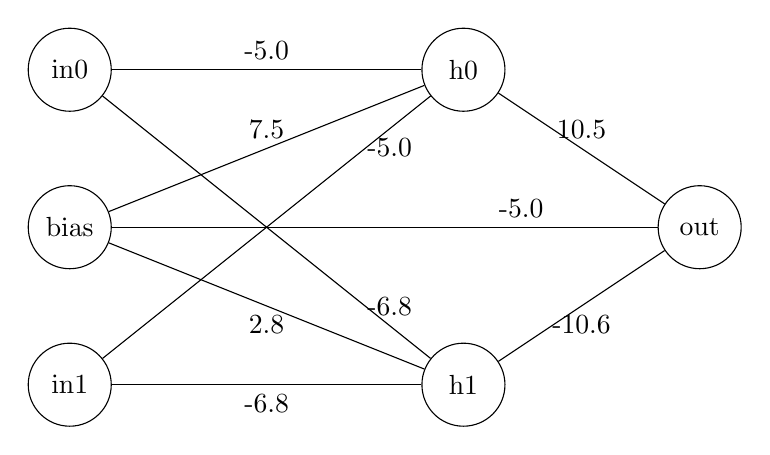
\begin{tikzpicture}
\tikzstyle{neuron}=[draw, circle, minimum size=30pt]

\draw (0,2) node[neuron] (bias) {bias};
\draw (0,4) node[neuron] (in0) {in0};
\draw (0,0) node[neuron] (in1) {in1};
\draw (5,4) node[neuron] (h0) {h0};
\draw (5,0) node[neuron] (h1) {h1};
\draw (8,2) node[neuron] (out) {out};

\draw (in0) edge node[above] {-5.0} (h0);
\draw (in0) edge node[very near end, above] {-6.8} (h1);
\draw (in1) edge node[very near end, below] {-5.0} (h0);
\draw (in1) edge node[below] {-6.8} (h1);
\draw (h0) edge node[above] {10.5} (out);
\draw (h1) edge node[below] {-10.6} (out);
\draw (bias) edge node[above] {7.5} (h0);
\draw (bias) edge node[below] {2.8} (h1);
\draw (bias) edge node[near end, above] {-5.0} (out);
\end{tikzpicture}
\end{center}

Based on these weights, this network solves XOR as follows.

Clearly, when both input nodes are on (ie. 1), each hidden node will compute the
sigmoid of negative weighted sums that are large in magnitude, thus both hidden nodes will be inactive.
When both hidden nodes are inactive, the weighted value coming into the output node is just -5, which when
passed into the sigmoid function approximates 0, the correct output - XOR(1,1) = 0!

When both input nodes are off (ie. 0), both hidden nodes will receive positive weighted sums of a large magnitude,
thus both hidden nodes will be active. However, the weight of the edge between h0 and the output node and
the weight of the edge between h1 and the output node are of almost the same magnitude but the opposite sign,
so they cancel each other out. This leaves us with a weighted value of approx. -5 (from the edge coming from the bias),
thus the sigmoid again approximates 0, the correct output - XOR(0,0) = 0!

When one input node is on (either in0 or in1 is 1), both hidden nodes will receive the weighted sum of
an incoming edge from an input node (-5 and -6.8 respectively) and the incoming edge from the bias
node (7.5 and 2.8 respectively). This yields a weighted sum of +2.5 for h0 and -4.0 for h1. Passing these
values into the sigmoid function, h0 is clearly active (large positive value) and h1 is clearly inactive
(large negative value). When the activation value of h0 is combined with the large positive weight of the edge between h0
and the output node, this yields a large positive value which far outweighs the -5 component from the
incoming bias edge. When passed into the sigmoid, this approximates 1, the correct output - XOR(1,0) = 0 and XOR(0,1) = 0!

\end{document}
